\documentclass[runningheads]{llncs}
\usepackage[T1]{fontenc}
\usepackage{graphicx}
\usepackage{placeins}
\usepackage{changepage}
\usepackage{multirow}
\usepackage{amsmath}
\usepackage{amssymb}
\usepackage{algorithm}
\usepackage{algpseudocode}
\usepackage{booktabs}
\usepackage{subcaption}

\begin{document}

\title{Evolving Patch-Level Attention via Genetic Algorithm for AI-Generated Image Detection Under Cross-Generator Shift}

\titlerunning{Evolving Patch-Level Attention for AI Image Detection}

\author{Alk{\i}m G\"onen\c{c} Efe \and Sarp S\"unb\"ul}

\authorrunning{A. G. Efe \and S. S\"unb\"ul}

\institute{Department of Computer Engineering, Faculty of Engineering and Architecture, \.{I}zmir Katip \c{C}elebi University, 35620 \.{I}zmir, Turkey}

\maketitle

\begin{abstract}
Detecting AI-generated images becomes substantially harder when the test images come from generators unseen during training. We address this cross-generator distribution shift by introducing a pipeline in which a genetic algorithm evolves conditional rulesets that produce per-image soft attention masks over a patch grid, highlighting regions whose patch-level features---gradient statistics, noise residuals, texture, and spectral properties---best separate AI-generated from human-generated content. These masks are provided as a secondary input channel to a CNN classifier alongside the raw image, allowing the network to leverage both pixel-level patterns and structured feature-level attention. To isolate the contribution of the evolutionary search, we compare three models sharing an identical CNN backbone: a baseline with no masking, a model with GA-evolved masks, and a control model with random masks matched to the same sparsity distribution. In-distribution, all three models converge to comparable accuracy ($\sim$98.4\%), confirming that masking offers no advantage when generator-specific artifacts are directly learnable from pixels. Under cross-generator shift, the GA-masked model achieves 78.6\% accuracy and 88.9\% precision compared to 77.7\% accuracy and 83.4\% precision for the baseline, while the random-masked control performs at or below the baseline (77.5\% accuracy, 71.8\% F1), confirming that the advantage stems from the structure of patch selection rather than sparsity or the additional input channel. JPEG robustness analysis reveals that the masking channel introduces sensitivity to lossy compression, a trade-off inherent to reliance on fine-grained spatial statistics. These results demonstrate that evolutionary feature masking captures generator-invariant discriminative structure that random selection does not, with the benefit emerging specifically under distribution shift.

\keywords{AI-generated image detection \and Genetic algorithm \and Feature masking \and Cross-generator generalization \and Distribution shift}
\end{abstract}

%% ====================================================================
\section{Introduction}
%% ====================================================================

The rapid advancement of generative models has made photorealistic synthetic imagery trivially producible. Diffusion-based architectures such as ADM~\cite{dhariwal2021diffusion} and GLIDE~\cite{nichol2022glide}, latent diffusion systems such as Stable Diffusion~\cite{rombach2022highresolution}, and autoregressive systems such as VQDM each produce distinct families of visual artifacts that are difficult to characterise with a single static detector. More recent systems such as DALL-E~3~\cite{betker2023dalle3}, Midjourney, and FLUX~\cite{flux2024} continue to push photorealism to the point where generated images are often indistinguishable from photographs by human observers, making this a moving-target problem in which each new generator family may invalidate existing detection strategies. Detection systems trained on one family of generators routinely fail when evaluated on images from generators unseen during training~\cite{zhu2023genimage}. This cross-generator distribution shift represents the central practical obstacle in the field: a detector that works only on known generators has limited real-world value.

Most existing detection pipelines pass entire images through a convolutional or transformer backbone and rely on the network to discover discriminative features on its own. A natural question arises from this setup: whether explicitly guiding the network to attend to specific spatial regions---patches that carry discriminative artifacts---can improve robustness to generator shift. The present work explores one instantiation of this idea. A genetic algorithm evolves conditional rulesets that, when applied to per-patch feature vectors, produce a per-image soft mask over a patch grid. The fitness function rewards rulesets whose selected patches maximise the statistical divergence between AI-generated and human-generated feature distributions. These masks are then provided as a second input channel to a convolutional neural network classifier alongside the raw image.

This work focuses on a specific question: whether structured, per-image algorithmic masking via genetic algorithm provides discriminative signals compared to random masking or no masking, and whether this advantage is more pronounced under cross-generator distribution shift than in-distribution. The experiments are designed to isolate this question through controlled comparison of three models sharing an identical CNN backbone, differing only in their masking strategy.

The remainder of this paper is organised as follows. Section~2 surveys related work in AI-generated image detection and evolutionary approaches. Section~3 describes the methodology in detail, including the feature extraction pipeline, genetic algorithm design, and CNN architecture. Section~4 presents the experimental setup, including dataset construction and hyperparameter configuration. Section~5 reports the results of four experiments. Section~6 discusses the implications and limitations of the findings.

%% ====================================================================
\section{Related Works}
%% ====================================================================

The detection of AI-generated images has been approached from several angles, including CNN-based classifiers, frequency-domain analysis, patch-level learning, and evolutionary computation. This section surveys representative works from each direction and identifies the gap that the present work addresses.

Bird and Lotfi~\cite{bird2023cifake} proposed a straightforward CNN classifier trained on the CIFAKE dataset, achieving approximately 92.9\% accuracy on 32$\times$32 real-versus-diffusion images. While effective within its training distribution, the static nature of the architecture means it cannot adapt its feature extraction strategy to new generators. The model learns generator-specific pixel-level patterns rather than more fundamental signatures of synthetic content, resulting in poor cross-generator transfer.

Liu et al.~\cite{liu2022detecting} took a different approach by leveraging frequency-domain noise patterns. They observed that authentic images share common noise characteristics in the frequency domain that GAN-generated or flow-based images lack, and trained a simple classifier on these patterns. While the single noise-residual feature is effective for certain generator families, it represents only one of many possible discriminative signals. The approach is limited by its reliance on a single statistical dimension.

Sinitsa and Fried~\cite{sinitsa2024fingerprint} introduced a model-specific fingerprint computed by averaging denoised residuals of generated images. This allows detection of images from a specific generator with very few training samples, but the method requires re-extraction of a new fingerprint for each previously unseen generator. The approach is inherently generator-specific rather than generator-agnostic.

The problem of patch-level feature utilisation has received direct attention in recent work. Yang et al.~\cite{yang2025panoptic} identified a ``Few-Patch Bias'' in naive detectors: networks tend to latch onto a small number of salient patches while ignoring the rest of the image. Their Panoptic Patch Learning framework uses random patch replacement and patch-wise contrastive learning to force the network to attend to all patches uniformly. The present work addresses the same underlying observation but from the opposite direction---rather than forcing uniform patch usage, it uses evolutionary optimisation to discover which patches actually carry the strongest discriminative signals.

Transformer-based approaches have also been explored. Liu et al.~\cite{liu2024fatformer} introduced FatFormer, which adds specialised forgery-aware adapter modules to a pretrained CLIP-ViT backbone. The method integrates image and frequency features and aligns them with text embeddings through language prompts. While effective, it depends on large pretrained models and does not provide explicit control over which spatial regions receive attention.

Epstein et al.~\cite{epstein2023online} studied detection in a continual learning setting, sequentially training on images from generator releases over time. Their work underscores the need for detectors that can adapt as new models appear, though their approach focuses on the learning regime rather than on feature engineering or spatial attention.

In the evolutionary computation domain, Lin et al.~\cite{lin2023genetic} developed a genetic programming framework that evolves tree-structured programs for interpretable AI-generated image detection. Their programs process images through four specialised layers: region detection, image filtering, feature extraction, and feature concatenation before SVM classification. While achieving competitive cross-generator performance (e.g., 95.67\% accuracy on StarGAN), their approach processes entire images through fixed pipelines rather than performing per-image spatial selection.

The present work uses evolutionary optimisation to evolve conditional rulesets that construct per-image attention masks from patch-level features. These masks are fed alongside the raw image into a standard CNN classifier. Because the ruleset and the classifier are separate components, the contribution of the evolutionary search can be isolated by comparing it against random masks of identical sparsity---a controlled experimental design that none of the surveyed works provide. This separation also means the approach is modular: the ruleset evolves on feature-level statistics independently of the CNN training loop, and the CNN receives both raw pixels and mask-weighted feature maps for its classification decision.

%% ====================================================================
\section{Methodology}
%% ====================================================================

The system operates in three sequential phases. Phase~1 optimises per-feature importance weights using Bayesian hyperparameter optimisation (Optuna~\cite{akiba2019optuna}), establishing which of the eight patch-level features carry the most discriminative information. Phase~2 evolves a set of conditional rules using a genetic algorithm implemented with the DEAP framework~\cite{fortin2012deap}; these rules are applied to patch-level features to produce a per-image soft mask over the patch grid. Phase~3 trains a convolutional neural network classifier that receives two inputs: the raw image and a feature map constructed from the mask-weighted patch features. Fig.~\ref{fig:pipeline} illustrates the overall architecture.

\begin{figure}[!htbp]
\centering
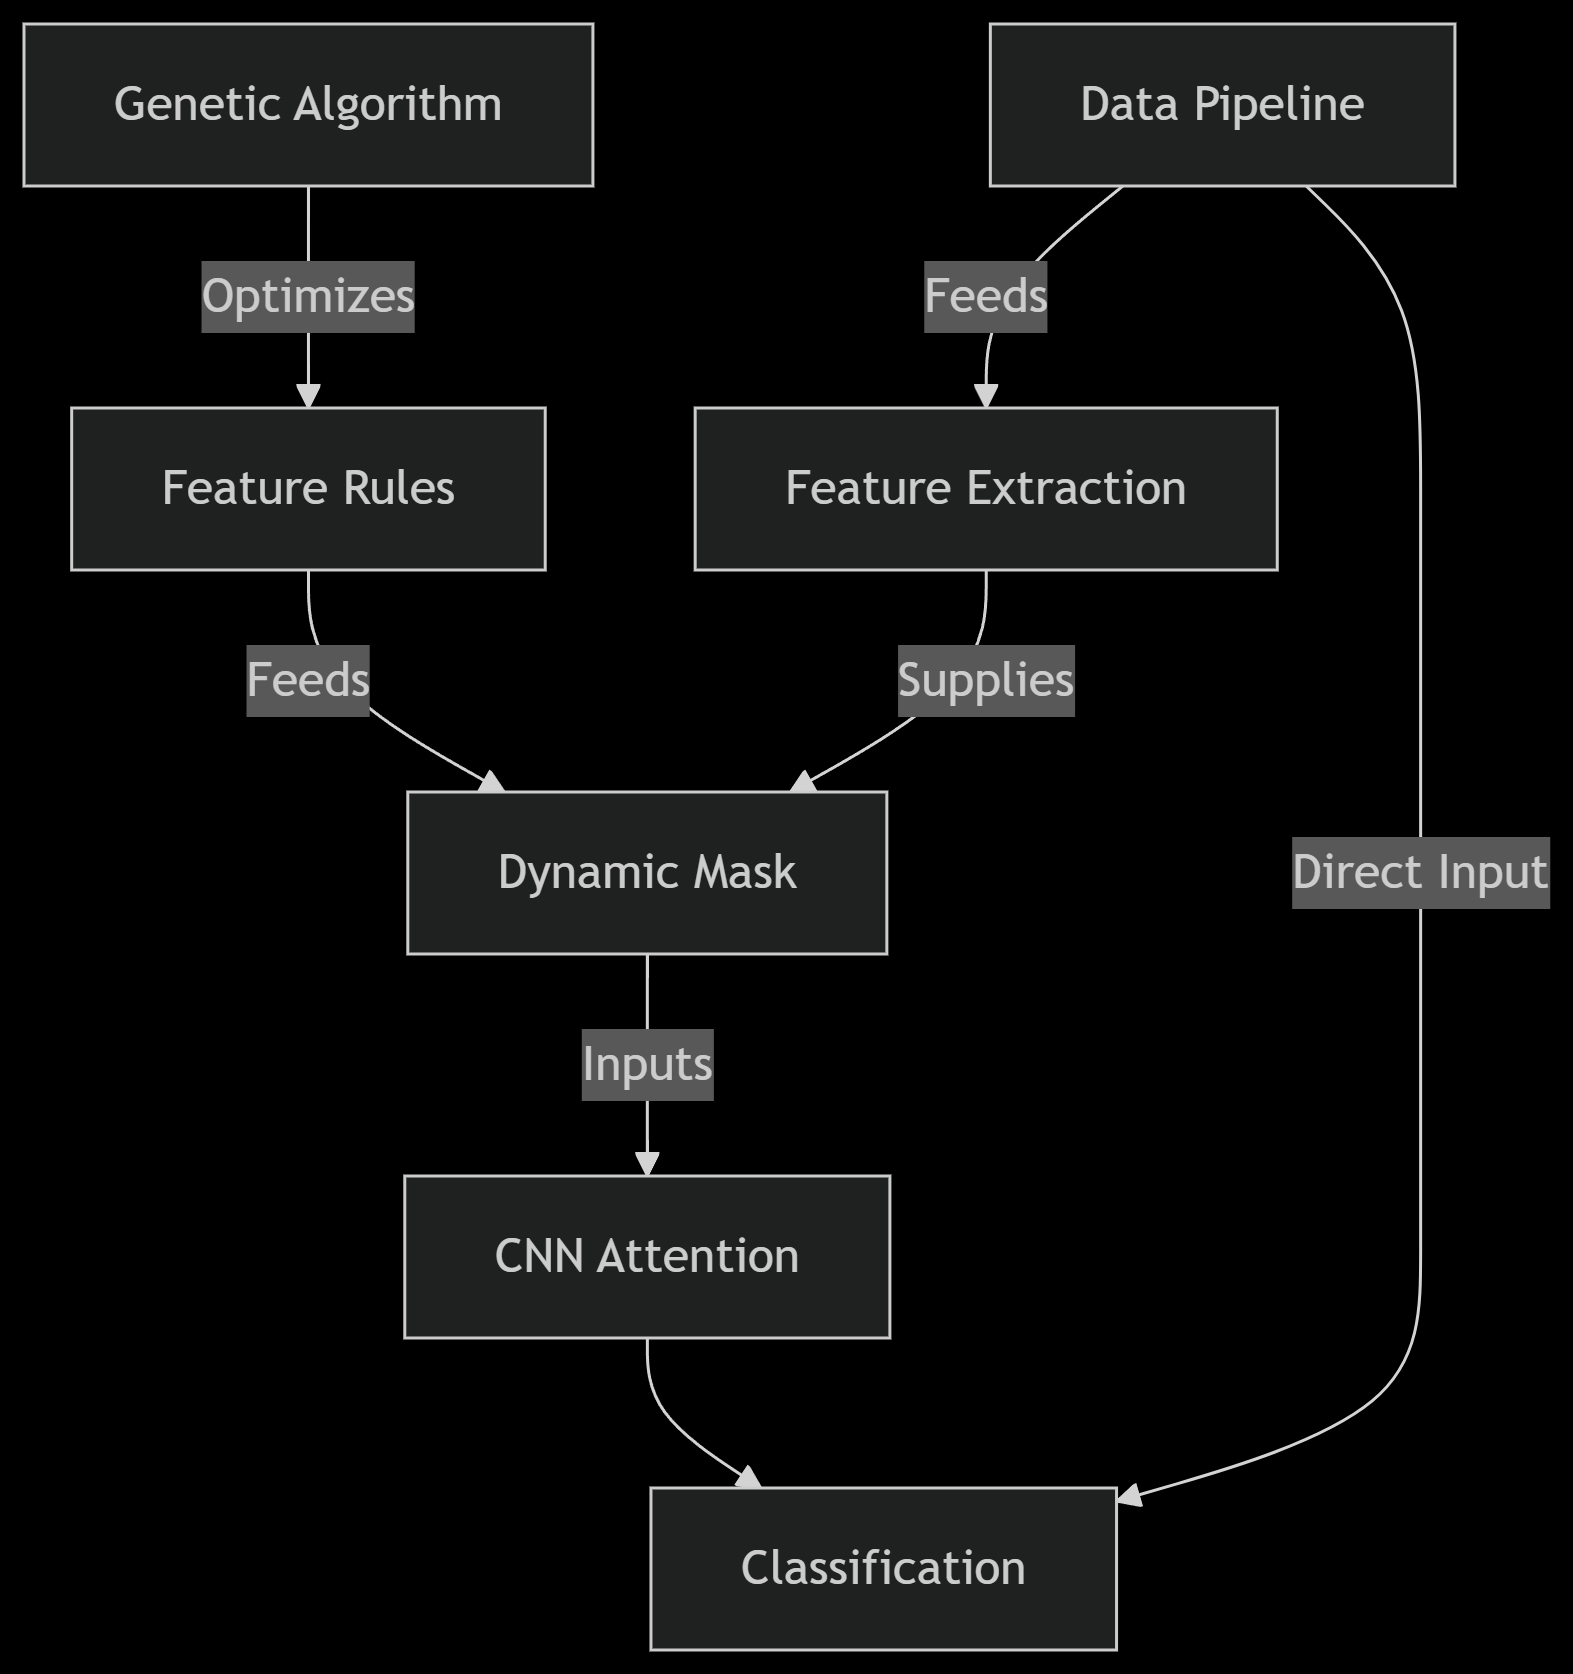
\includegraphics[width=0.55\textwidth]{deepseek_mermaid_20250619_c4d3df}
\caption{Architecture of the proposed pipeline. The data pipeline feeds images both directly to the CNN and through the feature extraction module. The genetic algorithm optimises conditional rules that generate dynamic per-image masks from extracted features. These masks modulate the feature maps before they enter the CNN attention mechanism, where they are fused with the image branch for final classification.}
\label{fig:pipeline}
\end{figure}

Three model variants sharing the same CNN architecture and training protocol are compared. The baseline (no mask) model receives only the raw image, with no feature maps and no masking. The GA-masked model receives the raw image alongside feature maps produced by applying evolved GA rules to per-patch features. The random-masked model (control) receives the raw image alongside feature maps produced by applying random binary masks with the same sparsity distribution as the GA masks, isolating the effect of structured selection from the effect of sparsity itself.

\subsection{Patch Feature Extraction}

Each input image $I \in \mathbb{R}^{256 \times 256 \times 3}$ is divided into a grid of non-overlapping $8 \times 8$~pixel patches via TensorFlow's \texttt{tf.image.extract\_patches} operation, yielding a $32 \times 32$ patch grid containing 1{,}024 patches per image. For each patch, eight scalar features are computed by averaging per-pixel feature maps over the patch area, producing a feature tensor $\mathbf{F} \in \mathbb{R}^{32 \times 32 \times 8}$.

The eight features, implemented as TensorFlow-native operations for full GPU execution, are described below along with their mathematical formulations.

The gradient perfection metric applies Sobel operators~\cite{kanopoulos1988design} to compute horizontal and vertical gradients:
\begin{equation}
G_x = \begin{bmatrix} -1 & 0 & 1 \\ -2 & 0 & 2 \\ -1 & 0 & 1 \end{bmatrix}, \quad
G_y = \begin{bmatrix} -1 & -2 & -1 \\ 0 & 0 & 0 \\ 1 & 2 & 1 \end{bmatrix}
\end{equation}
The gradient magnitude $M = \sqrt{G_x^2 + G_y^2}$ is computed per pixel, and the feature value is the variance of $M$ over the patch. Unnaturally smooth transitions in AI-generated images produce lower gradient variance than natural camera images.

The noise uniformity feature applies a Laplacian filter~\cite{gonzalez2002digital} to isolate high-frequency noise:
\begin{equation}
L = \begin{bmatrix} 0 & 1 & 0 \\ 1 & -4 & 1 \\ 0 & 1 & 0 \end{bmatrix}, \quad \text{Noise} = \text{Var}(\nabla^2 I)
\end{equation}
The variance of the Laplacian response captures the absence of natural sensor noise that is characteristic of generated images.

The symmetry feature measures horizontal and vertical pixel-difference symmetry by computing the normalised correlation between opposite halves of the patch:
\begin{equation}
S = \frac{\sum (I_{\text{left}} \odot I_{\text{right}})}{\|I_{\text{left}}\| \cdot \|I_{\text{right}}\|}
\end{equation}
Generative models, particularly those conditioned on symmetric prompts, exhibit bias toward unnatural levels of spatial symmetry.

The LBP texture feature implements Local Binary Patterns~\cite{ojala2002multiresolution} by comparing each pixel $p_c$ with its eight neighbours $p_i$ in a circular arrangement:
\begin{equation}
\text{LBP} = \sum_{i=0}^{7} s(p_i - p_c) \cdot 2^i, \quad s(x) = \begin{cases} 1 & x \geq 0 \\ 0 & \text{otherwise} \end{cases}
\end{equation}
The resulting histogram entropy characterises local texture regularity.

The colour saturation feature converts the patch to HSV colour space and computes the variance of the saturation channel:
\begin{equation}
\sigma_S^2 = \frac{1}{HW} \sum_{i,j} (S_{ij} - \mu_S)^2
\end{equation}
AI-generated images often exhibit unnaturally uniform colour distributions that produce low saturation variance.

The hash complexity feature computes a DCT-based perceptual hash by reducing the patch to an $8 \times 8$ grayscale representation, computing the Discrete Cosine Transform, and measuring the entropy of bit transitions in the resulting hash. This captures overall synthetic signatures related to the spectral structure of the patch.

The GLCM texture feature computes Gray-Level Co-occurrence Matrix~\cite{haralick1973textural} contrast and homogeneity scores. The co-occurrence matrix tabulates the frequency of pixel-intensity pairs at a fixed spatial offset, and the derived statistics capture second-order texture properties.

The local entropy feature computes the Shannon entropy of quantised grayscale intensity histograms within each patch:
\begin{equation}
H = -\sum_{k} p_k \log_2 p_k
\end{equation}
where $p_k$ is the probability of intensity bin $k$. Low-entropy patches indicate regions of unnaturally flat intensity.

Feature values are dynamically normalised using per-feature 99th-percentile scales computed from the training set, ensuring consistent ranges across datasets and preventing outlier domination. These scales are computed once during the preprocessing stage and serialised for consistent application during evaluation and inference.

\subsection{Genetic Algorithm}

The genetic algorithm is implemented using the DEAP framework~\cite{fortin2012deap}, a Python library for evolutionary computation that provides infrastructure for population management, tournament selection, crossover, mutation, and Hall of Fame elitism. The GA operates on the precomputed patch feature tensor $\mathbf{F}$ and evolves a population of candidate rulesets, each representing a strategy for constructing per-image attention masks.

Each individual in the population encodes a variable-length set of conditional rules (up to 40 rules, with typically 10 active at initialisation) as a tensor of shape $[\text{max\_rules}, 4]$, where each row encodes a rule $r_i = [\text{feature\_index},\; \text{threshold},\; \text{operator},\; \text{action}]$. The feature index selects one of the eight feature channels, the threshold is a scalar in $[0, 1]$, the operator is either greater-than or less-than, and the action is either include or exclude. Rules with a feature index of $-1$ are treated as inactive padding.

For a given image with patch features $\mathbf{F} \in \mathbb{R}^{32 \times 32 \times 8}$, each rule votes independently on each patch. The final soft mask is computed as the difference of normalised include and exclude vote fractions:
\begin{equation}
m(h,w) = \text{clip}\!\left(\frac{\sum_{r \in R_{\text{incl}}} \mathbb{1}[r \text{ fires at } (h,w)]}{|R_{\text{incl}}|} - \frac{\sum_{r \in R_{\text{excl}}} \mathbb{1}[r \text{ fires at } (h,w)]}{|R_{\text{excl}}|},\; 0,\; 1\right)
\label{eq:softmask}
\end{equation}
where $R_{\text{incl}}$ and $R_{\text{excl}}$ denote the subsets of include and exclude rules respectively. This formulation produces a soft mask: patches with unanimous include votes receive weight 1.0, patches with mixed signals receive fractional weights, and patches with net exclusion receive weight 0.0. The entire mask generation procedure is implemented as a single vectorised TensorFlow graph via \texttt{@tf.function} to allow batched processing on GPU without Python-level loops.

The fitness of an individual is a weighted combination of four objectives:
\begin{equation}
\text{Fitness} = w_d \cdot D_{\text{gated}} + w_e \cdot E + w_c \cdot C + w_s \cdot S
\label{eq:fitness}
\end{equation}

The divergence score $D$ is the primary fitness component and measures how well the mask-selected patches separate AI-generated from human-generated images across the evaluation batch. It combines Fisher Discriminant Ratio (FDR)~\cite{fisher1936use} and Bhattacharyya distance~\cite{bhattacharyya1943measure} into a composite score weighted by the per-feature importance weights from Phase~1:
\begin{equation}
D = \sum_f w_f \left(0.6 \cdot (1 - e^{-\text{FDR}_f}) + 0.4 \cdot (1 - e^{-\text{BC}_f})\right)
\label{eq:divergence}
\end{equation}
The FDR for each feature channel $f$ is computed as $\text{FDR}_f = (\mu_{f}^{\text{ai}} - \mu_{f}^{\text{human}})^2 / (\sigma_{f,\text{ai}}^2 + \sigma_{f,\text{human}}^2 + \epsilon)$, where $\mu$ and $\sigma^2$ are the mean and variance of the masked feature vectors for each class. The Bhattacharyya distance uses a Gaussian approximation combining both shape and Mahalanobis terms: $\text{BC}_f = 0.5 \cdot \ln\!\left(\frac{\bar{\sigma}_f^2}{\sigma_{f,\text{ai}} \cdot \sigma_{f,\text{human}}}\right) + 0.25 \cdot \frac{(\mu_f^{\text{ai}} - \mu_f^{\text{human}})^2}{\sigma_{f,\text{ai}}^2 + \sigma_{f,\text{human}}^2}$. Both measures are saturated through the $1 - e^{-x}$ transform to prevent unbounded growth. The divergence score is gated by a sparsity floor: $D_{\text{gated}} = D \cdot \min(\text{sparsity}/0.10, 1)$, which prevents degenerate masks that select fewer than 10\% of patches from receiving inflated divergence scores.

The efficiency score $E$ applies a quadratic penalty outside a target sparsity range:
\begin{equation}
E = \max\!\left(1 - \left(\frac{\max(|\text{sparsity} - t| - r, 0)}{0.4}\right)^{\!2},\; 0\right)
\end{equation}
where $t$ is the target sparsity and $r$ is the tolerance radius. This produces a plateau of perfect efficiency within the target range and smooth degradation outside it.

The connectivity score $C$ measures spatial coherence of selected patches using convolution with a cross-shaped 3$\times$3 kernel. For each selected patch, the kernel counts the number of selected neighbours (up to 4). The connectivity score is the mean ratio of actual to maximum possible connections across the batch, normalised to $[0, 1]$. This encourages spatially contiguous mask regions rather than scattered selections.

The simplicity score $S$ penalises rule complexity beyond the number of features: $S = 1 - \max(\text{active\_rules} - 8, 0) / (\text{max\_rules} - 8)$. This prevents the GA from overfitting through excessive rule counts.

An inactive-weight penalty is applied to individuals that ignore high-weight features. The penalty sums the Phase~1 weights of features not utilised by any active rule and is phased in proportionally to the divergence score to avoid suppressing immature but promising individuals early in evolution.

The selection mechanism uses tournament selection~\cite{goldberg1991comparative} with configurable tournament size. Crossover operates by swapping rule subsets between two parent individuals at a randomly chosen crossover point. Mutation introduces controlled perturbations to thresholds, flips comparison operators and actions, and can add or remove rules within predefined limits. Elitism preserves top individuals via a Hall of Fame with similarity-based deduplication, where similarity is computed as the fraction of matching rule components between two individuals.

\subsection{Random Mask Generator (Control)}

The random mask control is implemented as a subclass of the feature pipeline that replaces the GA mask generation step with a stochastic process. For each image, each patch is independently selected with probability equal to the mean sparsity of the GA masks (approximately 16.4\%). Seeds are derived deterministically from per-image feature sums via \texttt{tf.random.stateless\_uniform} to ensure that different images receive different masks while maintaining reproducibility across runs. The random pipeline reuses all other infrastructure---feature extraction, caching, normalisation, and dataset preparation---identically to the GA pipeline, ensuring that the only difference between the two conditions is the structure of the mask.

\subsection{CNN Architecture}

All three model variants share the same CNN architecture, implemented using TensorFlow and Keras~\cite{tensorflow2015whitepaper}. The image branch consists of three convolutional blocks, each containing a 2D convolutional layer with $3 \times 3$ kernels (32, 64, and 128 filters respectively), ReLU activation, $2 \times 2$ max-pooling, and batch normalisation~\cite{ioffe2015batch}.

For the GA-masked and random-masked models, a parallel feature branch processes the $256 \times 256 \times 8$ feature map (mask-weighted patch features upsampled to image resolution) through a mirrored three-block architecture with the same filter progression. A $1 \times 1$ convolutional attention gate on the image branch produces spatial weights in $[0, 1]$ that modulate the feature branch output via element-wise multiplication. The modulated features are then element-wise multiplied with the image branch activations (cross-attention) and added back to the image branch through a residual connection. This mechanism allows the CNN to selectively integrate information from the mask-weighted features where the image content suggests relevance.

After the attention fusion, a fourth convolutional layer (128 filters, $3 \times 3$) feeds into $2 \times 2$ max-pooling, batch normalisation, and global average pooling. Two dropout layers with rates determined by hyperparameter optimisation precede a dense layer and a sigmoid output. The baseline model replaces the attention fusion with an additional convolutional layer to maintain comparable model capacity. Training uses the Adam optimiser~\cite{kingma2015adam} with binary cross-entropy loss, mixed-precision arithmetic (float16 compute, float32 accumulation) via \texttt{LossScaleOptimizer} for GPU efficiency, learning rate reduction on plateau, and early stopping. L2 kernel regularisation is applied to all convolutional and dense layers.

%% ====================================================================
\section{Experimental Setup}
%% ====================================================================

\subsection{Dataset}

All experiments use the GenImage benchmark~\cite{zhu2023genimage}, a large-scale dataset specifically designed for AI-generated image detection research. GenImage encompasses multiple generative model families and provides standardised train/test splits across generator types.

Three generators are used for training: ADM~\cite{dhariwal2021diffusion}, GLIDE~\cite{nichol2022glide}, and Wukong. From each generator, 10{,}000 AI-generated and 10{,}000 real images are sampled, yielding a balanced training set of 30{,}000 images. For in-distribution evaluation, a stratified 20\% held-out validation split is drawn from the same generators (5{,}000 images). For cross-generator evaluation, two unseen generators are used: Stable Diffusion v4 (sdv4) and VQDM, with 2{,}500 AI-generated and 2{,}500 real images per generator (5{,}000 images total). All images are centre-cropped and resized to $256 \times 256$ pixels and normalised to $[0, 1]$. The dataset is loaded through a custom CSV-indexed pipeline built on TensorFlow's \texttt{tf.data} API, with stratified sampling to maintain balanced class distributions throughout all processing stages.

\subsection{Hyperparameter Configuration}

The GA hyperparameters were selected through Bayesian optimisation using Optuna~\cite{akiba2019optuna}. Table~\ref{tab:ga_params} lists the final GA configuration. The population of 120 individuals evolves for 80 generations across three independent runs, and the ruleset with the highest fitness is selected for Phase~3.

\begin{table}[!htbp]
\centering
\caption{Genetic algorithm hyperparameters. Values were selected through Bayesian optimisation.}
\label{tab:ga_params}
\begin{tabular}{@{}lc@{}}
\toprule
Parameter & Value \\
\midrule
Population size & 120 \\
Number of generations & 80 \\
Rules per individual (initial) & 10 \\
Maximum possible rules & 40 \\
Crossover probability & 0.814 \\
Mutation probability & 0.216 \\
Tournament size & 3 \\
Number of elites (Hall of Fame) & 4 \\
Inactive weight penalty & 0.032 \\
Target sparsity & 0.260 \\
Sparsity radius & 0.105 \\
Number of GA runs & 3 \\
Best fitness achieved & 0.325 \\
\bottomrule
\end{tabular}
\end{table}

CNN hyperparameters were optimised for the baseline and GA mask modes through separate Optuna studies targeting cross-generator validation accuracy. The random mask model reuses the GA mask hyperparameters to ensure a controlled comparison where architecture and training regime are identical, isolating the effect of mask structure. Table~\ref{tab:cnn_params} presents the resulting configurations.

\begin{table}[!htbp]
\centering
\caption{CNN hyperparameters per mask mode. Values were selected through Bayesian optimisation targeting cross-generator validation accuracy.}
\label{tab:cnn_params}
\begin{tabular}{@{}lccc@{}}
\toprule
Parameter & Baseline & GA Mask & Random Mask \\
\midrule
Learning rate & 0.00215 & 0.00109 & 0.00109 \\
Dropout (layer 1) & 0.381 & 0.168 & 0.168 \\
Dropout (layer 2) & 0.149 & 0.344 & 0.344 \\
Dense units & 832 & 960 & 960 \\
L2 regularisation & $1.79 \times 10^{-5}$ & $7.57 \times 10^{-4}$ & $7.57 \times 10^{-4}$ \\
Optimiser & Adam & Adam & Adam \\
HPO val.\ accuracy & 0.782 & 0.793 & 0.749 \\
\bottomrule
\end{tabular}
\end{table}

\subsection{Feature Weight Optimisation}

Phase~1 of the pipeline determines the relative importance of each feature channel for separating AI-generated from human-generated images. An Optuna study optimises a set of eight feature weights by maximising a fusion fitness score that measures the overall discriminability of the weighted feature combination. Table~\ref{tab:feature_weights} presents the learned weights along with the achieved fusion fitness score.

\begin{table}[!htbp]
\centering
\caption{Learned feature weights from Phase~1 Bayesian optimisation. The fusion fitness score (0.368) measures the overall discriminability of the weighted feature combination on the training set.}
\label{tab:feature_weights}
\begin{tabular}{@{}lc@{}}
\toprule
Feature & Weight \\
\midrule
Noise uniformity & 0.318 \\
Gradient perfection & 0.220 \\
Hash complexity & 0.168 \\
Symmetry & 0.101 \\
LBP texture & 0.093 \\
Local entropy & 0.051 \\
Colour saturation & 0.034 \\
GLCM texture & 0.014 \\
\midrule
Fusion fitness score & 0.368 \\
\bottomrule
\end{tabular}
\end{table}

Noise uniformity receives the highest weight (0.318), consistent with the well-established observation that generative models produce unnaturally uniform noise distributions compared to natural camera sensor noise~\cite{liu2022detecting}. Gradient perfection ranks second (0.220), capturing the overly smooth gradient transitions characteristic of diffusion model outputs. Hash complexity and symmetry contribute moderately, while GLCM texture and colour saturation contribute minimally, suggesting that co-occurrence statistics and colour distributions are less discriminative at the $8 \times 8$ patch scale used in this study.

\subsection{Fitness Weights}

The four components of the GA fitness function (Eq.~\ref{eq:fitness}) are weighted as shown in Table~\ref{tab:fitness_weights}. The divergence score receives the dominant weight (0.75), reflecting the primary objective of maximising inter-class feature separation. Efficiency and simplicity each receive a weight of 0.10 to prevent degenerate or overly complex solutions, while connectivity receives a minimal weight of 0.05 as a soft encouragement toward spatially coherent masks.

\begin{table}[!htbp]
\centering
\caption{Fitness function component weights used in the genetic algorithm.}
\label{tab:fitness_weights}
\begin{tabular}{@{}lc@{}}
\toprule
Component & Weight \\
\midrule
Divergence score ($D$) & 0.75 \\
Efficiency score ($E$) & 0.10 \\
Connectivity score ($C$) & 0.05 \\
Simplicity score ($S$) & 0.10 \\
\bottomrule
\end{tabular}
\end{table}

\subsection{Training Protocol}

All CNN models are trained for a maximum of 50 epochs with a batch size of 64 and a fixed random seed of 42. Early stopping monitors validation accuracy with a patience of 20 epochs, restoring the best weights upon termination. Learning rate reduction on plateau halves the learning rate when validation loss stagnates for 5 consecutive epochs. Mixed-precision training uses float16 computation with float32 weight accumulation, managed through TensorFlow's \texttt{LossScaleOptimizer} to maintain numerical stability. Training uses a single NVIDIA GPU, with feature extraction batches processed through TensorFlow's \texttt{tf.data} pipeline with prefetching. For the GA and random models, patch features are precomputed and cached to disk as NumPy memory-mapped arrays before training begins, eliminating redundant feature extraction across epochs.

%% ====================================================================
\section{Results}
%% ====================================================================

\subsection{In-Distribution Evaluation}

All three models are trained on images from ADM, GLIDE, and Wukong, and evaluated on a held-out validation split drawn from the same generators. This experiment measures baseline classification ability when the test distribution matches the training distribution. Table~\ref{tab:indist} presents the results.

\begin{table}[!htbp]
\centering
\caption{In-distribution evaluation. All models are trained and tested on ADM, GLIDE, and Wukong.}
\label{tab:indist}
\begin{tabular}{@{}lcccc@{}}
\toprule
Model & Accuracy & F1 Score & Precision & Recall \\
\midrule
Baseline (no mask) & 0.9832 & 0.9833 & 0.9801 & 0.9864 \\
GA mask             & 0.9842 & 0.9841 & 0.9927 & 0.9756 \\
Random mask         & 0.9846 & 0.9845 & 0.9887 & 0.9804 \\
\bottomrule
\end{tabular}
\end{table}

All three models perform comparably, with accuracy differences within 0.14 percentage points. Neither masking strategy provides a meaningful advantage when the test set is drawn from the same generators used for training. This outcome is expected: when the CNN can already learn generator-specific artifacts directly from pixel patterns, the auxiliary masking signal has little room to add value. The GA-masked model achieves marginally higher precision (99.3\%) at the cost of slightly lower recall (97.6\%), indicating a tendency toward fewer but more confident positive predictions.

Fig.~\ref{fig:training_indist} shows the training history for the baseline model in the in-distribution setting. Training accuracy converges smoothly toward 99\%, while validation accuracy exhibits characteristic oscillation around 90--97\% due to the relatively small validation set and the batch normalisation statistics mismatch between training and evaluation modes. The gap between training and validation loss indicates moderate overfitting, which is mitigated by early stopping.

\begin{figure}[!htbp]
\centering

\includegraphics[width=\textwidth]{training_history_none__train_ADM_glide_wukong__test_ADM_glide_wukong}
\caption{Training history for the baseline (no mask) model in the in-distribution setting. Left: accuracy over epochs. Right: loss over epochs. The validation curve oscillation is typical for this dataset and model scale.}
\label{fig:training_indist}
\end{figure}

\subsection{Cross-Generator Generalisation}

Models trained on ADM, GLIDE, and Wukong are evaluated on Stable Diffusion v4 and VQDM, generators never seen during training. This experiment represents the core test of the paper's claim. Table~\ref{tab:crossgen} presents the results, and Fig.~\ref{fig:confusion_crossgen} shows the confusion matrices for all three models.

\begin{table}[!htbp]
\centering
\caption{Cross-generator evaluation. Models are trained on ADM, GLIDE, and Wukong; tested on sdv4 and VQDM.}
\label{tab:crossgen}
\begin{tabular}{@{}lcccc@{}}
\toprule
Model & Accuracy & F1 Score & Precision & Recall \\
\midrule
Baseline (no mask) & 0.7768 & 0.7559 & 0.8340 & 0.6912 \\
GA mask             & 0.7864 & 0.7539 & 0.8891 & 0.6544 \\
Random mask         & 0.7750 & 0.7181 & 0.9611 & 0.5732 \\
\bottomrule
\end{tabular}
\end{table}

\begin{figure}[!htbp]
\centering
\begin{subfigure}[b]{0.32\textwidth}
    
\includegraphics[width=\textwidth]{confusion_matrix_none__train_ADM_glide_wukong__test_sdv4_vqdm}
    \caption{Baseline}
\end{subfigure}
\hfill
\begin{subfigure}[b]{0.32\textwidth}
    
\includegraphics[width=\textwidth]{confusion_matrix_ga__train_ADM_glide_wukong__test_sdv4_vqdm}
    \caption{GA mask}
\end{subfigure}
\hfill
\begin{subfigure}[b]{0.32\textwidth}
    
\includegraphics[width=\textwidth]{confusion_matrix_random__train_ADM_glide_wukong__test_sdv4_vqdm}
    \caption{Random mask}
\end{subfigure}
\caption{Confusion matrices for the cross-generator evaluation. The baseline misclassifies 30.9\% of AI images as human. The GA model misclassifies 34.6\% of AI images but produces fewer false positives (8.2\% vs.\ 13.8\%). The random model achieves 97.7\% specificity but fails to detect 42.7\% of AI images.}
\label{fig:confusion_crossgen}
\end{figure}

The GA-masked model achieves the highest overall accuracy (78.6\%) compared to the baseline (77.7\%) and random masking (77.5\%). The margin is approximately one percentage point over the baseline, which is modest but aligns with our claim that structured masking provides additional discriminative signal under distribution shift.

The three models exhibit markedly different precision--recall trade-offs under shift. The confusion matrices in Fig.~\ref{fig:confusion_crossgen} illustrate this clearly. The random-masked model becomes extremely conservative: it correctly rejects 97.7\% of human images (only 58 false positives out of 2{,}500) but fails to detect 42.7\% of AI-generated images (1{,}067 false negatives). The GA-masked model sits in between, with 91.8\% specificity and 65.4\% sensitivity. The baseline has the most balanced profile, with 86.2\% specificity and 69.1\% sensitivity.

The random-masked model performs at or slightly below the baseline in both accuracy and F1 score (71.8\% vs.\ 75.6\%). This result confirms that the GA mask's advantage is not simply due to sparsity-induced regularisation or the provision of an extra input channel. The specific structure of patch selection is what matters.

The contrast between in-distribution and cross-generator results is informative. In-distribution, the GA mask's advantage over random masking is negligible (less than 0.1\% accuracy). Under cross-generator shift, the gap grows to approximately 1.1\% in accuracy and 3.6\% in F1 score. This pattern supports our claim that the advantage of structured masking is more pronounced under distribution shift.

Under cross-generator shift, all three models exhibit a substantial accuracy drop of approximately 20 percentage points compared to in-distribution performance, reflecting the inherent difficulty of the cross-generator task. The GA-masked model achieves the smallest absolute drop (19.8 pp) compared to the baseline (20.6 pp) and random masking (21.0 pp).

Fig.~\ref{fig:training_crossgen} shows the training history for the GA-masked model in the cross-generator setting. The divergence between training and validation curves is more pronounced than in the in-distribution case, reflecting the fundamental difficulty of the cross-generator task.

\begin{figure}[!htbp]
\centering

\includegraphics[width=\textwidth]{training_history_ga__train_ADM_glide_wukong__test_sdv4_vqdm}
\caption{Training history for the GA-masked model evaluated on the cross-generator test set. The large gap between training accuracy ($\sim$98\%) and validation accuracy ($\sim$70--78\%) reflects the distribution shift between training generators and the unseen sdv4/VQDM test generators.}
\label{fig:training_crossgen}
\end{figure}

\subsection{JPEG Robustness}

Each trained model is evaluated on JPEG-compressed versions of the test images at quality levels 100 through 10 (in steps of 10). For the GA and random models, patch features are recomputed from the compressed images and the same mask generation procedures are applied. Table~\ref{tab:jpeg} summarises accuracy at selected JPEG quality levels, and Fig.~\ref{fig:jpeg_robustness} presents the full degradation curves.

\begin{table}[!htbp]
\centering
\caption{Accuracy under JPEG compression at selected quality levels. ``Drop'' is the accuracy reduction from the clean (uncompressed) evaluation.}
\label{tab:jpeg}
\begin{tabular}{@{}ll ccc ccc@{}}
\toprule
& & \multicolumn{3}{c}{In-Distribution} & \multicolumn{3}{c}{Cross-Generator} \\
\cmidrule(lr){3-5} \cmidrule(lr){6-8}
Quality & & None & GA & Random & None & GA & Random \\
\midrule
Clean & Acc.  & .983 & .984 & .985 & .777 & .786 & .775 \\
100   & Acc.  & .822 & .811 & .837 & .731 & .705 & .630 \\
70    & Acc.  & .730 & .631 & .680 & .638 & .625 & .520 \\
50    & Acc.  & .703 & .596 & .654 & .623 & .606 & .512 \\
30    & Acc.  & .676 & .559 & .636 & .608 & .581 & .504 \\
10    & Acc.  & .576 & .506 & .567 & .566 & .542 & .500 \\
\midrule
Q50 & Drop  & .280 & .388 & .331 & .153 & .180 & .263 \\
\bottomrule
\end{tabular}
\end{table}

\begin{figure}[!htbp]
\centering
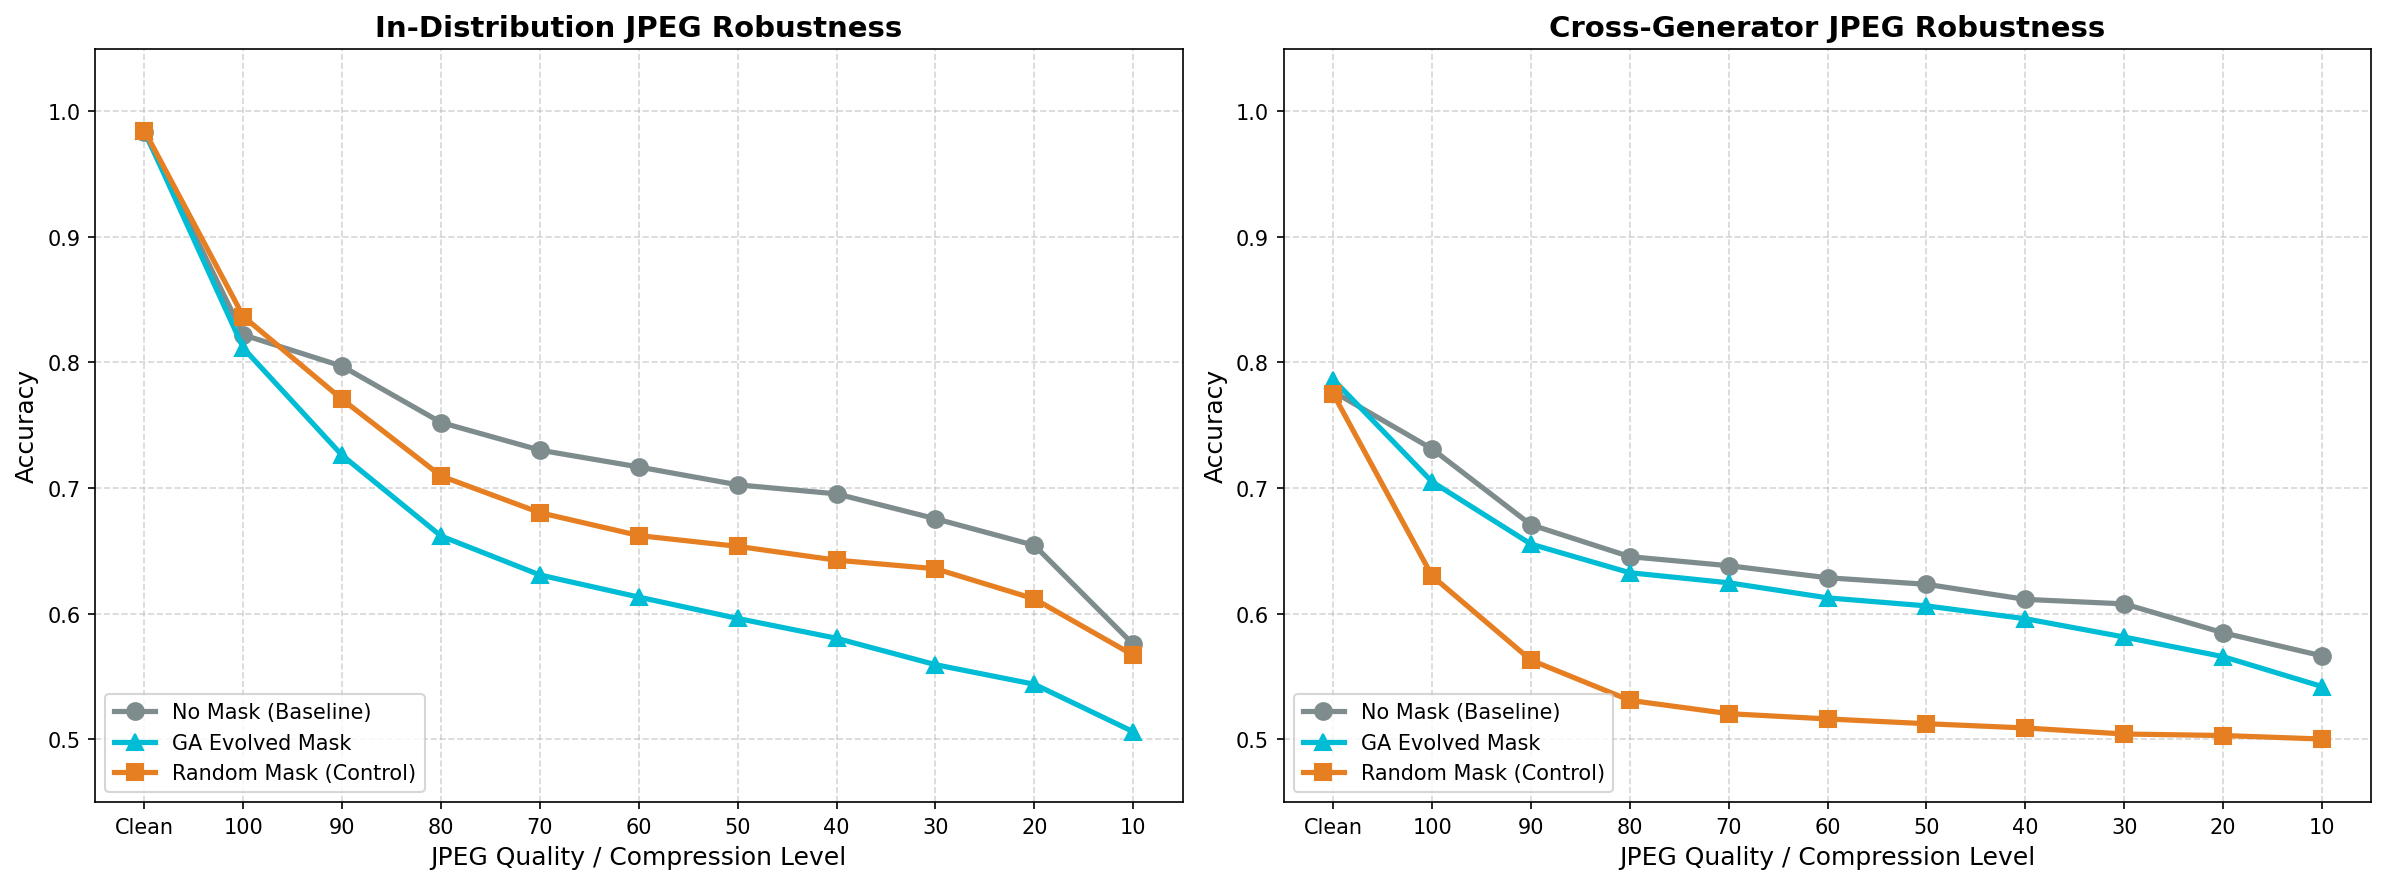
\includegraphics[width=\textwidth]{jpeg_robustness_comparison}
\caption{Accuracy degradation under JPEG compression for all three models. Left: in-distribution setting. Right: cross-generator setting. The baseline (grey circles) degrades most gracefully in both settings. The GA model (teal triangles) degrades faster than the baseline but slower than the random model in the cross-generator setting. The random model (orange squares) collapses toward chance (50\%) in the cross-generator setting at high compression levels.}
\label{fig:jpeg_robustness}
\end{figure}

As shown in Fig.~\ref{fig:jpeg_robustness}, masking amplifies JPEG fragility. In the in-distribution setting, the GA model drops 38.8 percentage points at quality level 50, compared to 28.1 for the baseline and 33.1 for the random model. The patch-level features---particularly gradient perfection, noise uniformity, and hash complexity---are computed from local pixel statistics that JPEG quantisation destroys. When the model depends on these features through the masking channel, it suffers more when they are corrupted.

The cross-generator JPEG results reveal a more dramatic pattern. The random-masked model drops to 50.0\% accuracy at quality level 10, which is effectively chance-level performance on a balanced binary classification task. The GA model retains 54.2\% and the baseline retains 56.6\%. The baseline is the most JPEG-robust model overall, which is not surprising given that it learns directly from pixels and does not depend on an auxiliary feature channel sensitive to compression artifacts.

The absolute accuracy drops are smaller in the cross-generator setting because the models start from a lower baseline ($\sim$78\% vs.\ $\sim$98\%). The relative degradation, however, is comparable across settings. These results reveal a trade-off: the masking channel that provides modest gains in clean cross-generator accuracy introduces a new vulnerability to lossy compression.

\subsection{Mask Visualisation and Interpretability}

The GA-evolved masks exhibit a mean sparsity of 16.4\% ($\sigma = 12.4\%$), meaning that on average approximately 170 of the 1{,}024 patches are selected per image. Masks vary substantially across images: some images receive dense masks (above 40\% coverage) while others are sparsely masked (below 5\%). This per-image adaptivity is by design, as the rules fire differently depending on each image's patch feature distribution.

Fig.~\ref{fig:mask_comparison} presents a visual comparison of GA-evolved and random masks applied to the same image. The GA mask concentrates its selections on regions with complex structural content, particularly areas with edges, texture transitions, and fine detail. In contrast, the random mask distributes its selections uniformly across the image without regard to content. Both masks select a similar proportion of patches (12.0\% GA vs.\ 17.7\% random for this particular image), but the spatial structure differs fundamentally.

\begin{figure}[!htbp]
\centering
\begin{subfigure}[b]{\textwidth}
    
\includegraphics[width=\textwidth]{mask_ga__train_ADM_glide_wukong__test_sdv4_vqdm_sample003}
    \caption{GA-evolved mask (12.0\% coverage). Selections concentrate on structural edges and textured regions.}
\end{subfigure}
\\[0.5em]
\begin{subfigure}[b]{\textwidth}
    
\includegraphics[width=\textwidth]{mask_random__train_ADM_glide_wukong__test_sdv4_vqdm_sample003}
    \caption{Random mask (17.7\% coverage). Selections are distributed uniformly without content awareness.}
\end{subfigure}
\caption{Comparison of GA-evolved and random masks on the same image. Left column: original image. Centre: patch mask visualisation with green (GA) or yellow (random) indicating selected patches. Right: mask overlay on the original image. The GA mask exhibits spatial structure that correlates with image content, while the random mask does not.}
\label{fig:mask_comparison}
\end{figure}

Fig.~\ref{fig:mask_additional} shows an additional GA mask example on a different image, illustrating how the mask adapts to image content. In this case, the mask focuses on the subject's body and boundary regions---areas where generative models commonly introduce subtle artifacts in edge rendering and fine detail synthesis.

\begin{figure}[!htbp]
\centering

\includegraphics[width=\textwidth]{mask_ga__train_ADM_glide_wukong__test_sdv4_vqdm_sample000}
\caption{GA-evolved mask on a second sample image (2.7\% coverage). The sparse mask focuses on the subject boundary and areas of fine detail, which are common sites of generative artifacts.}
\label{fig:mask_additional}
\end{figure}

The evolved rules provide a degree of interpretability that is uncommon in learned attention mechanisms. Each rule operates on a named image-processing feature computed by a well-documented algorithm: a rule such as ``include patches where noise uniformity exceeds 0.73'' references the normalised Laplacian variance, where 0.73 corresponds to a specific point on the distribution of Laplacian responses scaled by the 99th-percentile value observed in the training set. The threshold can be mapped back to an absolute Laplacian variance value by multiplying by the stored scale factor. More broadly, the identity of the features selected by the rules is itself informative: the dominance of noise uniformity and gradient perfection in the evolved rulesets (as reflected by the Phase~1 feature weights in Table~\ref{tab:feature_weights}) indicates that the pipeline identifies noise residual patterns and gradient smoothness as the primary signals distinguishing AI-generated from human-generated patches. These features correspond to well-understood properties of generative models---the absence of natural sensor noise and the tendency toward overly smooth spatial transitions---providing an interpretable account of what the system considers a ``tell'' of synthetic origin.

%% ====================================================================
\section{Discussion}
%% ====================================================================

The experimental evidence supports our core claim with important caveats. GA-evolved masks provide a small discriminative advantage over both no masking and random masking under cross-generator shift, with approximately 1.0\% higher accuracy over the baseline, 1.1\% higher accuracy over random masking, and 3.6\% higher F1 score over random masking. The advantage is absent in-distribution, which aligns with our reasoning that explicit feature selection becomes more valuable when the model cannot rely on generator-specific pixel-level patterns. Random masking provides no benefit over the baseline, confirming that the GA's advantage stems from the structure of its patch selection rather than from sparsity or the additional input channel alone.

The precision--recall analysis reveals that the three models occupy different positions on the precision--recall curve under distribution shift. The random model achieves near-perfect specificity (97.7\%) at the cost of poor sensitivity (57.3\%), the GA model achieves a balance leaning toward specificity (91.8\% specificity, 65.4\% sensitivity), and the baseline achieves the most symmetric trade-off (86.2\% specificity, 69.1\% sensitivity). The masking signal biases the classifier toward conservatism, with the GA masks producing a more calibrated version of this bias than random masks.

The GA model is not robust to JPEG compression. In fact, it is less robust than the baseline. The masking mechanism introduces a dependency on patch-level features, and when those features are corrupted by lossy compression, the model suffers disproportionately. This is a direct consequence of our design: the features that enable the GA to construct informative masks---gradient statistics, noise residuals, frequency-domain properties---are computed from local pixel statistics that JPEG quantisation destroys. This trade-off between clean-image discriminability and compression robustness is inherent to any pipeline that relies on fine-grained spatial statistics, and its acceptability depends on the deployment scenario.

The current configuration reflects deliberate engineering decisions, each made under computational budget constraints. The 8$\times$8 pixel patch size was chosen to balance spatial granularity against the dimensionality of the feature tensor and the computational cost of per-patch feature extraction across thousands of images. At this resolution, generator artifacts that manifest at larger spatial scales---such as anatomical inconsistencies in faces and hands---fall outside the scope of patch-level features. The eight handcrafted features were selected to cover complementary signal domains (spatial gradients, noise statistics, texture, colour, frequency), though they represent a subset of the possible discriminative signals available in each patch. The GA fitness function optimises for statistical feature divergence rather than downstream CNN accuracy; this was a deliberate decoupling that allows the GA to operate independently of the CNN training loop, substantially reducing the computational cost of the pipeline. The stochastic nature of genetic algorithms is a well-known consideration, addressed in our implementation through multiple independent GA runs, Hall of Fame elitism with similarity-based deduplication, and an inactive-weight penalty that encourages broad feature utilisation across the evolved rules.

The feature weight analysis in Table~\ref{tab:feature_weights} reveals that noise uniformity and gradient perfection together account for more than half of the total feature weight (53.8\%). The lower-weight features (GLCM at 1.4\%, colour saturation at 3.4\%) contribute minimally to the GA's mask construction, indicating that the discriminative signal at this patch scale is concentrated in noise and gradient statistics rather than in colour or co-occurrence texture measures.

This project is an undergraduate thesis exploration with a large number of interacting components: patch size, feature set, GA hyperparameters, CNN architecture, attention mechanism design, and fitness function formulation. Each of these axes was optimised within the available computational budget using Bayesian hyperparameter search, though exhaustive ablation across all combinations was not feasible. The results demonstrate that the general approach of using evolutionary search to construct per-image attention masks for a CNN produces measurable benefits under distribution shift, and provide a foundation for further investigation.

Future work could extend the approach in several directions. Multi-scale patch extraction would allow the system to capture artifacts that span larger spatial regions. Replacing handcrafted features with learned representations from a pretrained backbone (e.g., CLIP or DINOv2) would provide richer feature spaces for the GA to operate on. Aligning the GA fitness function with downstream CNN accuracy through a bilevel optimisation formulation would close the gap between mask quality and classification performance. Finally, compression-aware feature extraction---for example, computing features in a JPEG-invariant representation---could mitigate the compression fragility observed in our experiments.

\subsection{Design Constraints and Broader Considerations}

Several engineering constraints shaped the design of this system. The computational cost of the pipeline was a primary concern: per-patch feature extraction across tens of thousands of images, combined with a population-based evolutionary search over 80 generations, required careful budgeting of GPU compute time. This motivated the decoupled architecture in which the GA operates on precomputed feature statistics independently of the CNN training loop, and the use of mixed-precision arithmetic and NumPy memory-mapped caching to reduce memory pressure and accelerate data throughput. Reproducibility was addressed through fixed random seeds, deterministic mask generation via stateless random operations, serialisation of all hyperparameters and feature normalisation scales, and systematic logging of all experiment configurations and results.

From an ethical and social perspective, the detection of AI-generated images is directly relevant to combating visual misinformation, identity fraud, and non-consensual synthetic media. A detector that generalises across generator families---the central goal of this work---is more practically useful in these contexts than one that only identifies images from known sources. At the same time, detection tools carry dual-use risk: the same feature-level analysis that identifies synthetic content could theoretically be used to refine generators to evade detection. The interpretability of the evolved rulesets, discussed in Section~5.4, provides transparency into what the system considers discriminative, which supports accountability in deployment contexts.

This work relates to United Nations Sustainable Development Goal~16 (Peace, Justice and Strong Institutions), which includes targets for reducing corruption and ensuring public access to reliable information. Automated detection of AI-generated imagery contributes to the integrity of visual media in journalism, legal proceedings, and public discourse.

\subsection{Modern Methods and Tools}

The project draws on methods and tools from several areas of modern computer engineering. The genetic algorithm, implemented with the DEAP framework~\cite{fortin2012deap}, applies evolutionary computation principles---tournament selection~\cite{goldberg1991comparative}, crossover, mutation, and elitism---to a combinatorial optimisation problem over conditional rule spaces. Bayesian hyperparameter optimisation via Optuna~\cite{akiba2019optuna} was used to tune both the GA configuration and the CNN training parameters, replacing grid search with a sample-efficient tree-structured Parzen estimator. The CNN classifier was implemented in TensorFlow~\cite{tensorflow2015whitepaper} with Keras, using mixed-precision training (float16 compute with float32 accumulation) managed through \texttt{LossScaleOptimizer} for GPU efficiency. Feature extraction was implemented as a compiled TensorFlow graph (\texttt{@tf.function}) to enable batched GPU execution without Python-level loops. Data loading used \texttt{tf.data} pipelines with prefetching and parallel mapping. The attention fusion mechanism between image and feature branches uses $1 \times 1$ convolutional gating with residual connections, a design pattern drawn from modern attention-based architectures. All experiments were conducted on a single consumer-grade NVIDIA GPU, demonstrating that the approach is feasible without specialised compute infrastructure.

%% ====================================================================

\begin{thebibliography}{99}

\bibitem{dhariwal2021diffusion}
Dhariwal, P., Nichol, A.: Diffusion models beat GANs on image synthesis. In: Advances in Neural Information Processing Systems (NeurIPS), vol.~34, pp.\ 8780--8794 (2021)

\bibitem{nichol2022glide}
Nichol, A., Dhariwal, P., Ramesh, A., Shyam, P., Mishkin, P., McGrew, B., Sutskever, I., Chen, M.: GLIDE: Towards photorealistic image generation and editing with text-guided diffusion models. In: Proceedings of the 39th International Conference on Machine Learning (ICML), pp.\ 16784--16804 (2022)

\bibitem{rombach2022highresolution}
Rombach, R., Blattmann, A., Lorenz, D., Esser, P., Ommer, B.: High-resolution image synthesis with latent diffusion models. In: Proceedings of the IEEE/CVF Conference on Computer Vision and Pattern Recognition (CVPR), pp.\ 10684--10695 (2022)

\bibitem{betker2023dalle3}
Betker, J., Goh, G., Jing, L., et al.: Improving image generation with better captions. OpenAI Technical Report (2023)

\bibitem{flux2024}
Black Forest Labs: FLUX.1: Open-weight text-to-image model. Technical Report (2024)

\bibitem{bird2023cifake}
Bird, J., Lotfi, A.: CIFAKE: Image classification and explainable identification of AI-generated synthetic images. arXiv preprint arXiv:2303.14126 (2023)

\bibitem{liu2022detecting}
Liu, R., Zhang, X., Zhang, B., Dong, C., Lin, L.: Detecting generated images by real images. In: Proceedings of the European Conference on Computer Vision (ECCV), pp.\ 105--122 (2022)

\bibitem{sinitsa2024fingerprint}
Sinitsa, D., Fried, O.: Deep image fingerprint: Towards low-budget synthetic image detection and model lineage analysis. In: Proceedings of the IEEE/CVF Winter Conference on Applications of Computer Vision (WACV), pp.\ 1288--1297 (2024)

\bibitem{yang2025panoptic}
Yang, Y., Qiu, Y., Cui, P.: All patches matter, more patches better: Enhance AI-generated image detection via panoptic patch learning. arXiv preprint arXiv:2504.01396 (2025)

\bibitem{liu2024fatformer}
Liu, H., Wang, Y., Li, H., Zhao, R., Liu, L.: Forgery-aware adaptive transformer for generalizable synthetic image detection. In: Proceedings of the IEEE/CVF Conference on Computer Vision and Pattern Recognition (CVPR), pp.\ 2905--2914 (2024)

\bibitem{epstein2023online}
Epstein, D., Krause, M., Riemer, M., Manry, D., Wingate, D.: Online detection of AI-generated images. In: Proceedings of the IEEE/CVF International Conference on Computer Vision Workshops (ICCVW), pp.\ 2335--2344 (2023)

\bibitem{lin2023genetic}
Lin, M., Shang, L., Gao, X.: Enhancing interpretability in AI generated image detection with genetic programming. In: 2023 IEEE International Conference on Data Mining Workshops (ICDMW), pp.\ 371--378. IEEE (2023)

\bibitem{zhu2023genimage}
Zhu, M., Chen, H., Wang, Q., Li, L., Xue, Y., Wang, Z., Zheng, Z.: GenImage: A million-scale benchmark for detecting AI-generated image. arXiv preprint arXiv:2306.08571 (2023)

\bibitem{akiba2019optuna}
Akiba, T., Sano, S., Yanase, T., Ohta, T., Koyama, M.: Optuna: A next-generation hyperparameter optimization framework. In: Proceedings of the 25th ACM SIGKDD International Conference on Knowledge Discovery and Data Mining, pp.\ 2623--2631 (2019)

\bibitem{fortin2012deap}
Fortin, F.-A., De Rainville, F.-M., Gardner, M.-A., Parizeau, M., Gagn\'e, C.: DEAP: Evolutionary algorithms made easy. Journal of Machine Learning Research 13, 2171--2175 (2012)

\bibitem{tensorflow2015whitepaper}
Abadi, M., et al.: TensorFlow: Large-scale machine learning on heterogeneous systems. Software available from tensorflow.org (2015)

\bibitem{kingma2015adam}
Kingma, D.P., Ba, J.: Adam: A method for stochastic optimization. In: International Conference on Learning Representations (ICLR) (2015)

\bibitem{ioffe2015batch}
Ioffe, S., Szegedy, C.: Batch normalization: Accelerating deep network training by reducing internal covariate shift. In: Proceedings of the 32nd International Conference on Machine Learning (ICML), pp.\ 448--456 (2015)

\bibitem{kanopoulos1988design}
Kanopoulos, N., Vasanthavada, N., Baker, R.L.: Design of an image edge detection filter using the Sobel operator. IEEE Journal of Solid-State Circuits 23(2), 358--367 (1988)

\bibitem{gonzalez2002digital}
Gonzalez, R.C., Woods, R.E.: Digital Image Processing, 2nd edn. Prentice Hall (2002)

\bibitem{ojala2002multiresolution}
Ojala, T., Pietik\"ainen, M., M\"aenp\"a\"a, T.: Multiresolution gray-scale and rotation invariant texture classification with Local Binary Patterns. IEEE Transactions on Pattern Analysis and Machine Intelligence 24(7), 971--987 (2002)

\bibitem{haralick1973textural}
Haralick, R.M., Shanmugam, K., Dinstein, I.: Textural features for image classification. IEEE Transactions on Systems, Man, and Cybernetics SMC-3(6), 610--621 (1973)

\bibitem{fisher1936use}
Fisher, R.A.: The use of multiple measurements in taxonomic problems. Annals of Eugenics 7(2), 179--188 (1936)

\bibitem{bhattacharyya1943measure}
Bhattacharyya, A.: On a measure of divergence between two statistical populations defined by their probability distributions. Bulletin of the Calcutta Mathematical Society 35, 99--109 (1943)

\bibitem{goldberg1991comparative}
Goldberg, D.E., Deb, K.: A comparative analysis of selection schemes used in genetic algorithms. In: Foundations of Genetic Algorithms, vol.~1, pp.\ 69--93. Morgan Kaufmann (1991)

\end{thebibliography}

\end{document}
